\documentclass{beamer}
\setbeamercovered{transparent}
\beamertemplatenavigationsymbolsempty
\begin{document}

\begin{frame}{GNUTADEO}

  \begin{columns}
    \begin{column}{.5\textwidth}
      \begin{figure}
        \centering
        
\includegraphics[width=\textwidth]{img/gnutadeo.jpg}
      \end{figure}
    \end{column}

    \begin{column}{.5\textwidth}
      \begin{itemize}
      \item Colectivo de Software Libre.
      \item Promovemos el uso del Software Libre.
      \item Mapeo y generación de datos libres.
      \item \textbf{Instagram: @gnutadeo}
      \item \textbf{GitHub: github.com/GNUTADEO}
      \end{itemize}

    \end{column}
  \end{columns}


\end{frame}

\begin{frame}{Mapeo Árboles Colegio}

  \begin{columns}
    \begin{column}{.5\textwidth}
      \begin{figure}
        \centering
        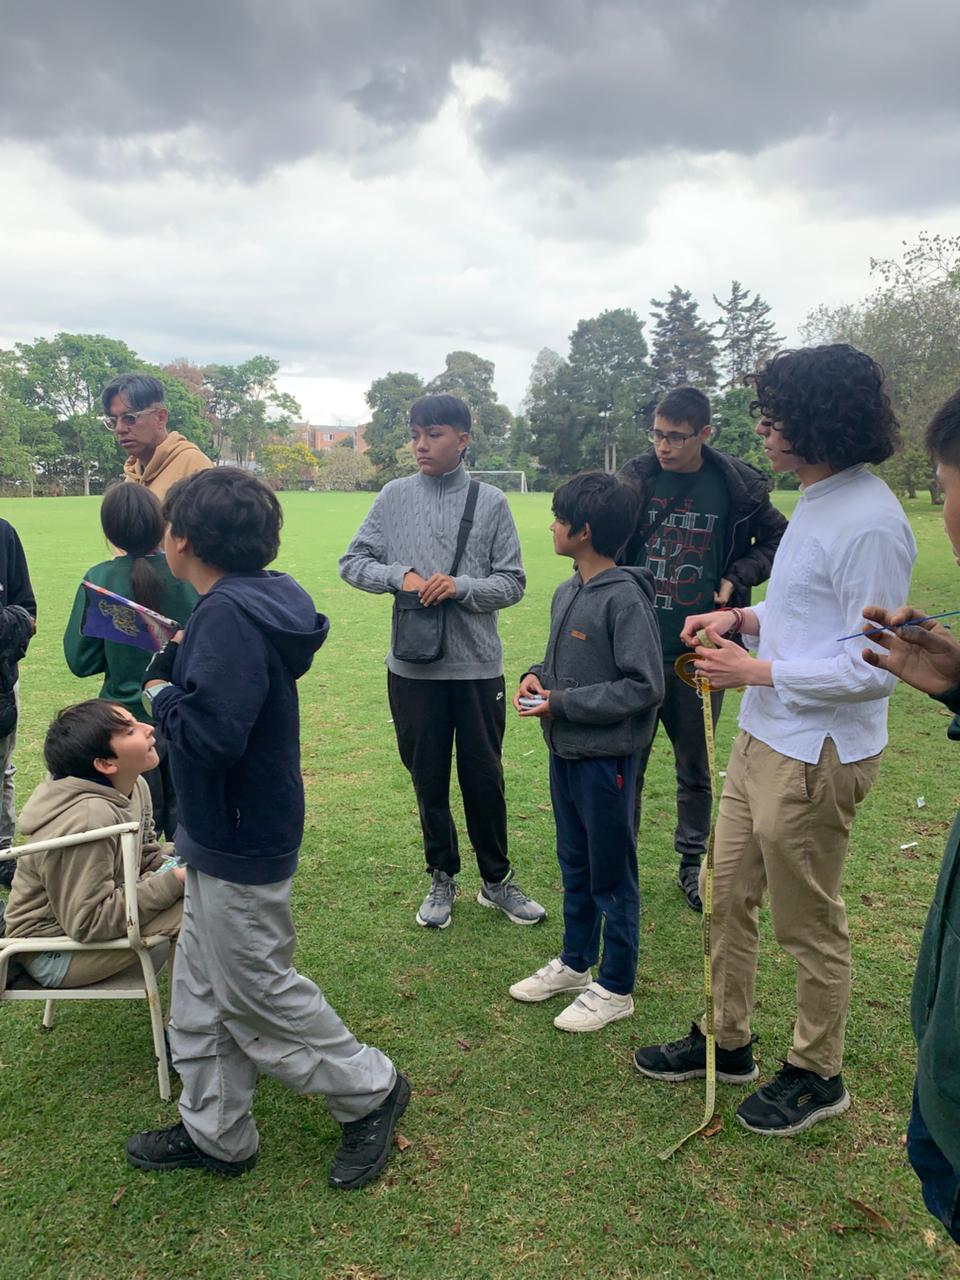
\includegraphics[width=\textwidth]{img/Mapeo1.jpg}
      \end{figure}
    \end{column}

    \begin{column}{.5\textwidth}
      \begin{figure}
        \centering
        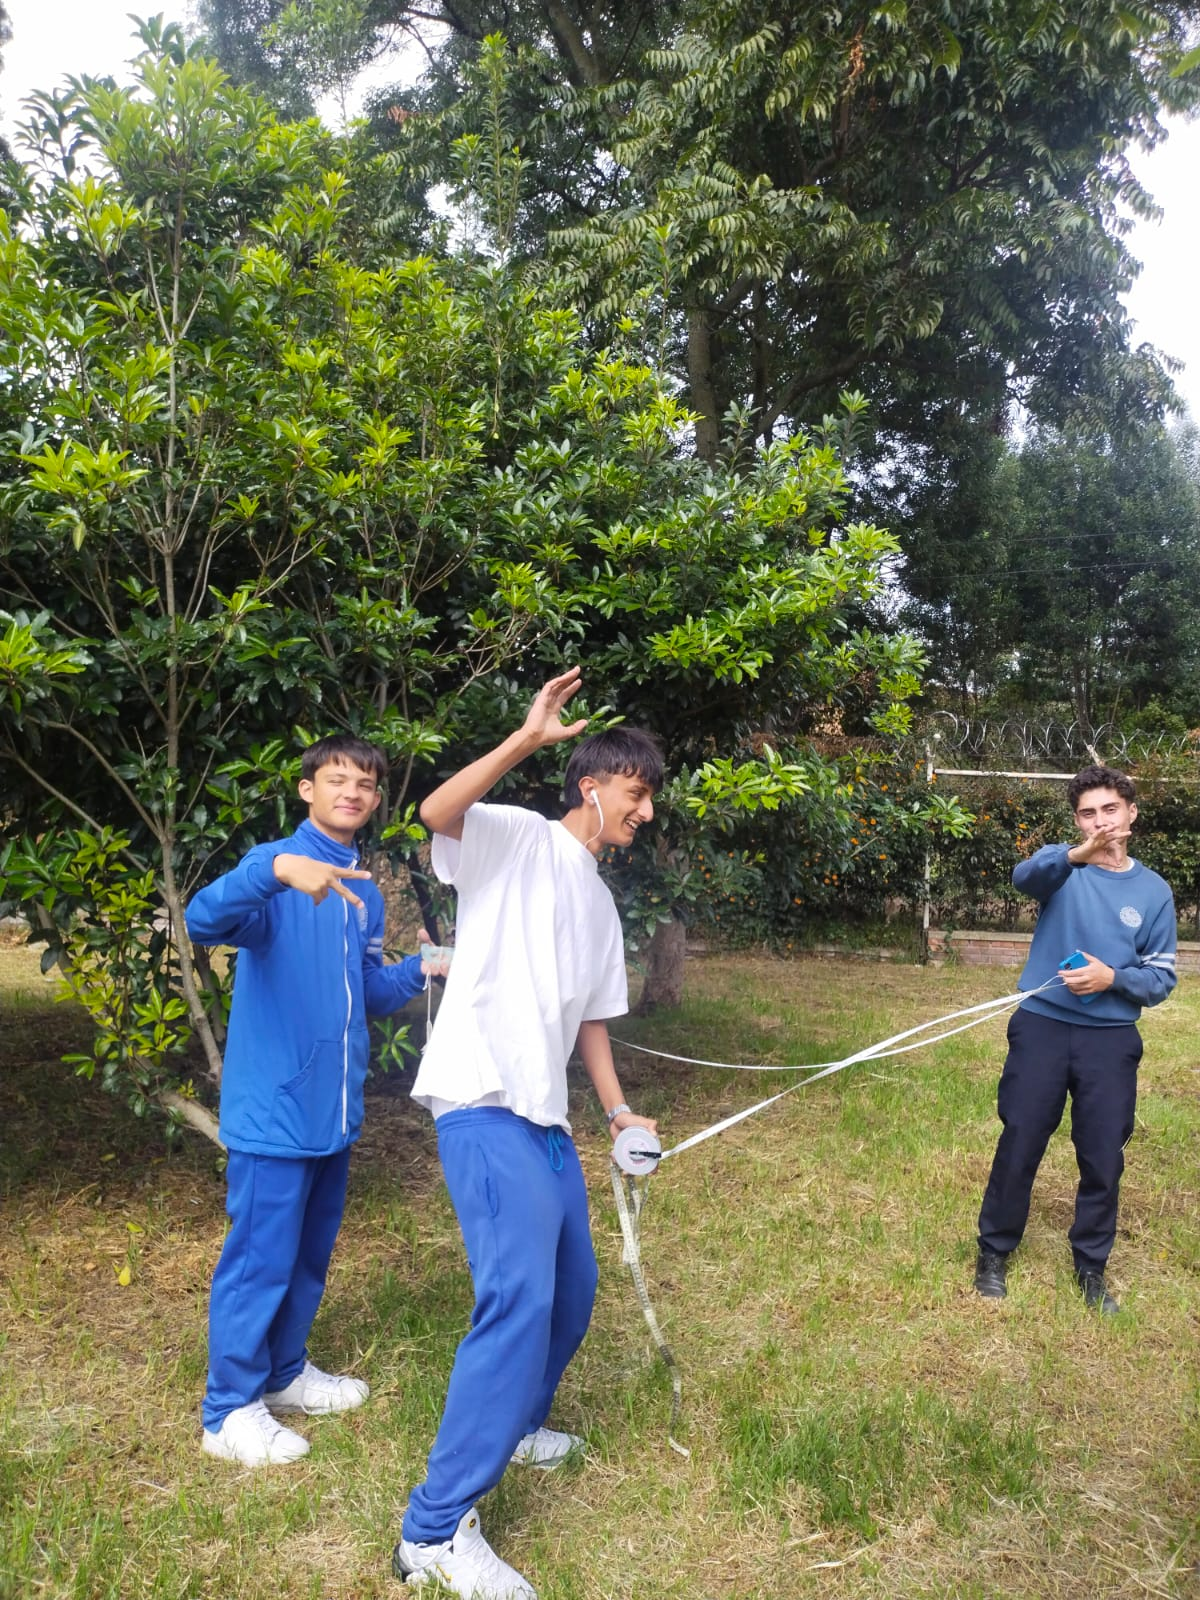
\includegraphics[width=\textwidth]{img/Mapeo2.jpg}
      \end{figure}
    \end{column}
  \end{columns}


\end{frame}



\begin{frame}{Mapatón Centro de Bogotá}

  \begin{columns}
    \begin{column}{.5\textwidth}
      \begin{figure}
        \centering
        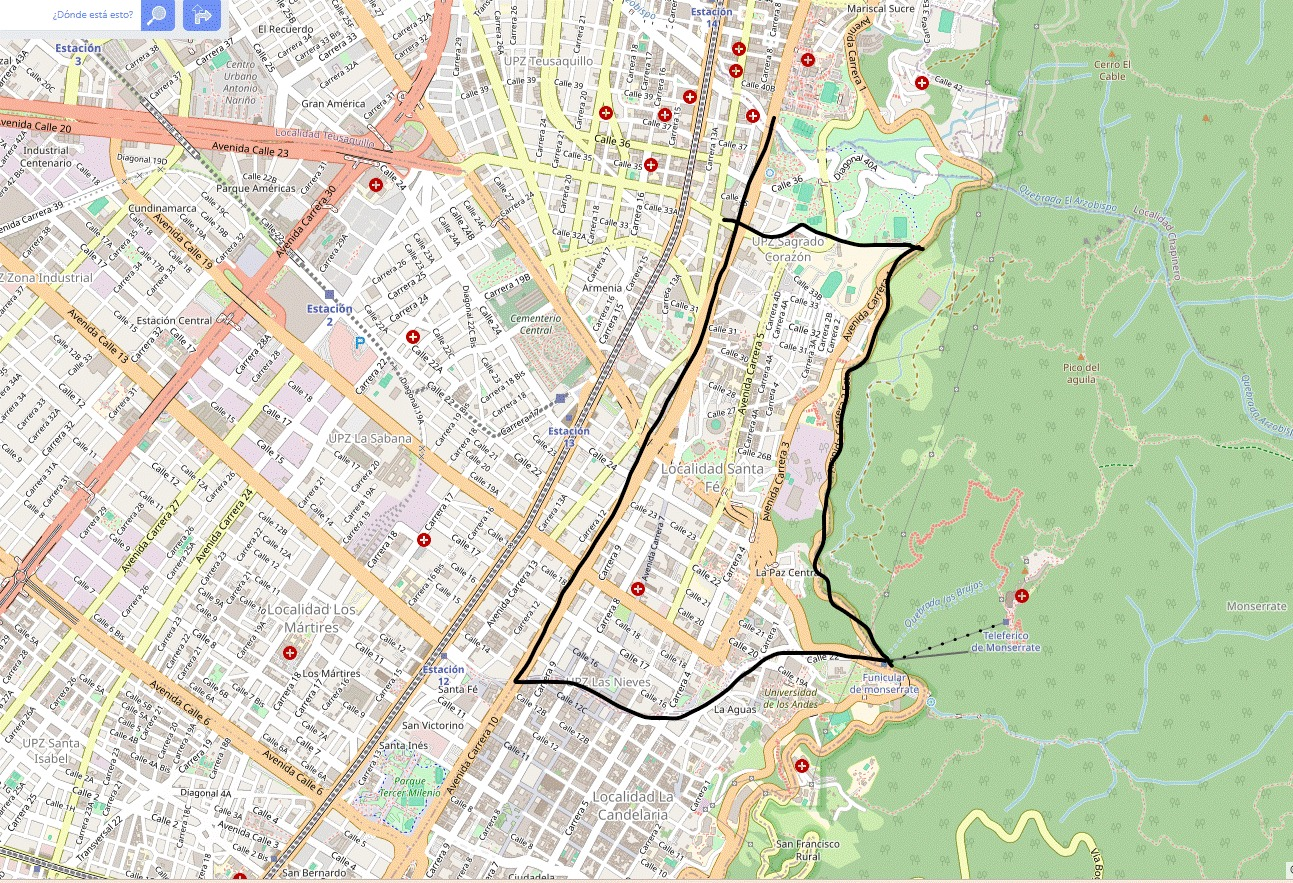
\includegraphics[width=\textwidth]{img/Mapaton.jpg}
      \end{figure}
    \end{column}

    \begin{column}{.5\textwidth}

      \begin{itemize}
      \item Mapatón por el centro de Bogotá.
      \item Alianza con TomTom y la Universidad Externado.
      \item Capítulo de YouthMappers: \textbf{TadeoMappers}.
      \end{itemize}
    \end{column}
  \end{columns}


\end{frame}


\begin{frame}{Asociación de Cartografía Colaborativa de Colombia (AC3)}

  \begin{columns}
    \begin{column}{.5\textwidth}
      \begin{figure}
        \centering
        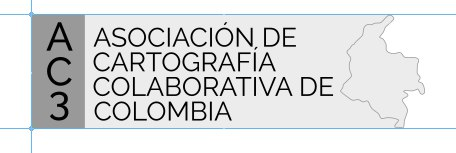
\includegraphics[width=\textwidth]{img/ac3.jpg}
      \end{figure}
    \end{column}

    \begin{column}{.5\textwidth}
      \begin{itemize}
      \item Empresa enfocada en generación de datos libres y otros servicios GIS.
      \item www.ac3.org.co
      \end{itemize}

    \end{column}
  \end{columns}


\end{frame}


\end{document}
